\documentclass[a4paper,12pt]{article}

% Packages
\usepackage[danish]{babel}
\usepackage{csquotes}
\usepackage{amsmath} % For math typesetting
\usepackage{amssymb} % For additional math symbols
\usepackage{geometry} % To adjust the page margins
\usepackage{graphicx} % To allow insert of pictures
\usepackage{float}    % Allows use of [H]
\usepackage{multicol}
\usepackage[table]{xcolor}
\usepackage{tikz}
\usepackage{caption}


% Bib 
\usepackage{biblatex} % Imports biblatex package
\addbibresource{ref.bib} % Import the bibliography file

% Custom commands
\newcommand{\myblock}[1]{#1}
\newcommand{\textbfit}[1]{\textbf{\textit{#1}}}

% Page margins
\geometry{margin=1in}


% Document title and author information
\title{Introduction Til Programmering \\
        Disposition 5 \\
        Designing Applications (Including design Patterns) \\
        Kapitel 15} 

\author{Joakim Iversen}
\date{03-12-2024}

\begin{document}

% Generate the title
    \maketitle
\newpage

\section*{Disposition:}
\begin{itemize}
    \item Finde klasserne
    \item CRC-kort
    \item Klasse desgin
    \item Design Patterns
\end{itemize}
\newpage


\begin{center}
    \textbfit{Kode eksempel:} \\
\end{center}

\section*{Notes:}

\subsection*{Kapitel 15 - Designing Applications:}
\subsubsection*{Main concepts:}
\begin{itemize}
    \item Discovering Classes
    \item CRC cards
    \item Designing interfaces
    \item Patterns
\end{itemize}
\subsubsection*{Notes:}
Blandt det største og vigtigste step til at lave en ny applikation - da det er her man undersøger hvordan forskellige klasser skal snakke sammen, hvordan metoder skal virke og hvilke feltvariabler der skal være de forskellige steder.

\textbf{Discovering Classes:} \\
En måde at finde ud af hvilke klasser, metoder og variabler man skal have er at bruge \textit{Udsagns-/navneords} metoden:

\begin{itemize}
    \item Beskriv med ord hvad programmet skal gøre
    \item Navneord = Ting/Klasser
    \item Udsagnsord = Handlinger/Metoder/Variabler
\end{itemize}

Når du har gjort dette kan du ende ud med fx følgende navneord og udsagnsord for et \textbfit{Biograf Booking System:}

\begin{table}[H]
    \centering
    \begin{tabular}{c c}
        \rowcolor{gray!30}
        \textbfit{Navneord} & \textbfit{Udsagnsord}  \\ \hline 
        Biograf Booking system  & Gemmer (sæde booking) \\
                                & Gemmer (Telefon nummer) \\
        Sæde booking            &  \\
        Biograf                 &  \\
        Sæde                    &  \\
        Række                   &  \\
        Kunde                   & Reservere (Sæde) \\
                                & Er givet (Række nummer, sæde nummer) \\
                                & Forspørge (Sæde booking) \\
        Række nummer            &  \\
        Sæde nummer             &  \\
        Forstilling             & Er skemalagt (i biograf) \\
        Film                    &  \\
        Dato                    &  \\
        Tid                     &  \\
        Telefon nummer          &
    \end{tabular}
    \caption{Tabel over ord fra en tekst der beskriver et biografs boking system. Måske skal hele tabellen ikke skrives op da dette vil tage for lang tid?}
\end{table}

Der er måske nogle ting her man ville undlade - Række, sæde nummer, osv... - fordi de virker til at være for basale ting til at have sin egen klasse. Men i dette skridt er det vigtigt ikke at undlade noget da vi ikke har nok information om ting til at bestemme hvad det er der skal være en klasse, og hvad bare skal være varibaler. Vi skal altså under dette skridt bare skrive \textit{alle} ord ned, uden at forholde os til kvaliteten af disse ord.

\textbf{CRC Cards:} \\
Nå vi har fundet vores navne- og udsagnsord i vores tekst er næste skridt at bruge CRC-kort \textit{(Class - Responsibility - Collaborators)}.
\begin{center}
    
    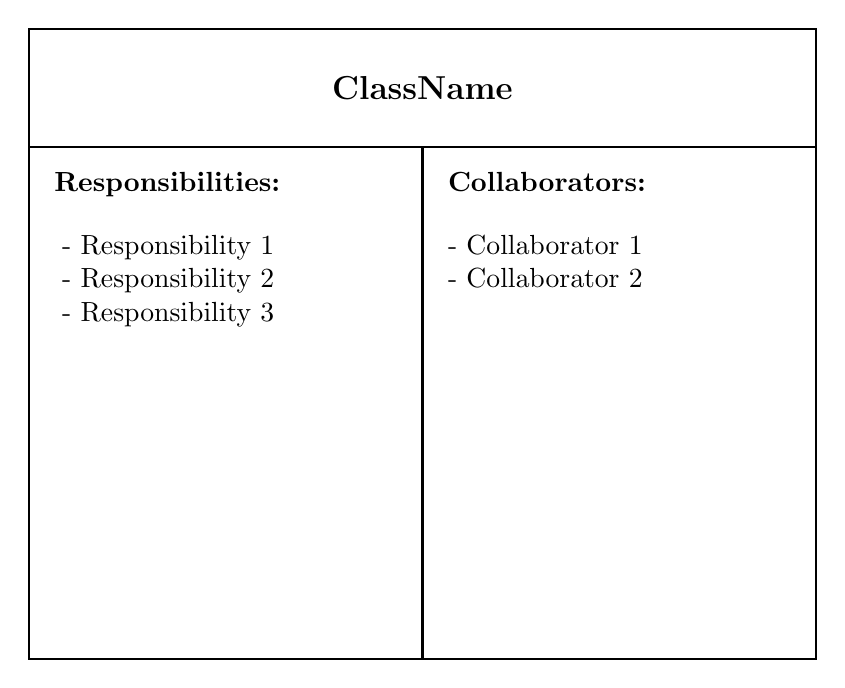
\begin{tikzpicture}
        % Outer rectangle for CRC card
        \draw[thick] (0, 0) rectangle (10, 8);
        
        % Class name section
        \draw[thick] (0, 6.5) -- (10, 6.5);
        \node[font=\large, anchor=center] at (5, 7.25) {\textbf{ClassName}};
        
        % Responsibilities section
        \draw[thick] (5, 6.5) -- (5, 0);
        \node[anchor=north west, font=\bfseries] at (0.2, 6.3) {Responsibilities:};
        \node[align=left, anchor=north west] at (0.3, 5.5) {
        - Responsibility 1\\
        - Responsibility 2\\
        - Responsibility 3
        };
        
        % Collaborators section
        \node[anchor=north west, font=\bfseries] at (5.2, 6.3) {Collaborators:};
        \node[align=left, anchor=north west] at (5.2, 5.5) {
            - Collaborator 1\\
            - Collaborator 2
            };
    \end{tikzpicture}
\end{center}
            
En af måderne du så vil kunne udfylde disse CRC kort på er ved at gennem gå et slags "rollespil". Man laver et fysisk kort for hver klasse hvor at - optimalt flere personer - tager et kort hver. Så gennemgår man flere forskellige scenarier hvor man siger hvad man gør. Samtidigt skriver man ned hvad det er ens klasser har brug for at kunne. Så hvis ens klasser spørger en anden klasse hvor mange "XXX" der er ledige, skriver man den klasse i Collaborators og så videre.

\textit{Eksempel:}
\begin{itemize}
    \item Brugeren skal finde alle forstillinger af en film i aften. Så vi kan i BiografBokkingSystem CRC-kort under responsibilities skrive \textit{Kan finde forstillinger ved titel og dag}. Vi kan også skrive \textit{film} udner deres Collaborators.
    \item   Vi skal så spørge os selv, hvordan finder systemet filmen? Hvem spørger den?
            En løsning er eventuelt at den selv gemmen en samling af film. Dette giver os en yderlige klasse: samlingen (Dette kan evt. implementeres senere ved brug af en ArrayList, LinkedList, HashSet eller en anden form for samling med yderligere metoder relevante til film. Den beslutning kan vi lave senere, vi skriver bare FilmCollection for nu). Dette er et eksempel på hvordan vi evt kan tilføje flere klasser mens vi "rollespiller" scenarier. Det kan altså ske at vi nogle gang skal tilføje ydderligere klasser end vi havde til at starte med, eller klasser som vi bare overså første fra teksten.
\end{itemize}

\textbf{Class Design:} \\
Nu har vi alle klasserne vi skal bruge og næste skridt er derfor at finde ud af hvad hver klasse skal kunne gøre. Dette kan vi gøre ved at lave et nyt "rollespil". Vi starter på præcis samme måde med at lave nye kort for hver klasse. Den her gang skal vi bare bruge de lidt mere formele beskrivelser af metodekald, parametre og retur værdier.

Dette fiver os nu overblik over hvilke metoder de forskellige klasser skal have, hvilke parametre disse skal tage og hvilke retur typer der skal være på dem. Ved brug af dette "dobbelte rollespil" er det altså muligt for os effektivt at undersøge hvordan vores programs akritektur skal opstilles og hvordan interaktionen skal kunne forgå imellem klasser.

\textbfit{Design Patterns: }\\
\begin{figure}[h]
    \begin{itemize}
        \item Decorator
        \item Singleton
        \item Factory Method
        \item Observer
    \end{itemize}
    \caption*{\textit{Nævn en eller to af dem her og lig op til spørgsmål omkring de andre}}
\end{figure}

En beskrivelse af et design pattern indeholder mindst:
\begin{itemize}
    \item Et navn der kan bruges i generel samtale omkring mønsteret
    \item En beskrivelse af problemmet mønsteret behandler (Ofte delt ind i sektioner som, hensigt, motivation og anvendelse)
    \item Beskrivelse af løsningen (ofte nævne struktur, deltagere og samarbejdspartnere)
    \item Konsekvenserne ved at bruge mønsteret (resultater og trade-offs)
\end{itemize}

\textbf{\fontsize{100pt}{10pt}\selectfont WHAT IS THIS!?}\\

\textbfit{Decorator: } \\
Decorator mønsteret omhandler at tilføje funktionalitet til et allerede eksisterende objekt. Vi antager at vi vil have et nyt objekt der reagere på de samme metode kald (Altså har det samme interface) men har tilføjet eller ændret lidt adfærd.

En måde at gøre dette på er ved hjælp af nedarvning. En subklasse vil måske overskrive implementationen af metoder og tilfje ydderlige metoder, men brugen af nedarvning er en statisk løsning: når skabt kan objekter ikke ændre deres adfærd.

Hvis du bruger decorator mønsteret laver du en subclass til klassen (Men ved brug af det reservered ord \textbf{implements} i setedet for extends) du vil ændre - ofte navngivet på formen \textit{xxxDecorator} - Herefter er det så decorator klassen som du laver subklasser til alt efter behov.

Herfra vil klienter snakke med objektet gennem decoratoren istedet for direkte til objektet. Et eksempel på dette kan fx være i UI designs hvor man vil have noget til at ske ved et knappe tryk - fx highlight af markeret tekst. Her vil trykket på knappen tilføje en decorator til den markerede tekst som highlighter det.

\textbfit{Singleton:} \\
Singleton mønsteret løser et problem hvor vi vil sikre os, at der kun en instans af et objekt til stede. Fx hvis vi laver et software development environment wil vi kun have en enkelt compiler eller debugger.

I Java vil vi kunne opnå dette ved at lave konstruktøren privat. Dette sikre sig at den ikke kna tilgås udenfor klassen, og vi vil derfor ikke kunne skabe flere instanser end dem vi laver i selve klassen. Herefter kan vi i singleton klassen skrive koden til at lave en enkelt instans af dette objekt og så give adgang til dette. 

Koden til dette vil kunne se sådan ud

\begin{verbatim}

public class Compiler {
    private static Compiler instance = new Compiler();

    public static Compiler getInstance() {
        return instance;
    }

    private Compiler() {
        ...
    }
}

\end{verbatim}

Det er ikke muligt for os at tilgå vores Compiler objekt her, uden at bruge metoden \textit{getInstance()}.

\textbfit{Factory Method: } \\
Factory mønsteret omhandler at man laver et generelt interface til at skabe objekter, men lader subklasser beslutte hvilke specifikke klasser der bliver skabt. Klienten forventer typisk at få givet en superklasse eller et interface af det efterspurgte objekts dynamiske type, og factory mønsteret tillader så specialisering af typen.

Et eksempel vil være i BlueJ's \textit{foxes-and-rabbits} eksempel. For at skille \textbf{simulator} klassen fra \textbf{fox} og \textbf{rabbit} klassen vil vi kunne implementere en \textbf{actorFactory} interface og så lave klasser der hverisær implementere dette interface (\textbf{foxFactory} og \textbf{rabbitFactory}). \textbf{Simulator} klassen vil så kun skulle gemme en samling af vores  \textbf{actorFactory} objekter og så individuelt spørge dem om at producere de nødvendige \textbf{foxFactory} og \textbf{rabbitFactory}.


\textbfit{Observer:} \\
???

\end{document}